\chapter*{LAMPIRAN}

\newappendix{Dokumentasi}

\begin{figure}[!h]
    \includegraphics[width=.8\linewidth, center]{images/lampiran/documentation/validation.JPG}
    \caption{Validasi akurasi pembacaan alat oleh PT Bisma Jaya selaku mitra dan PT Pertamina Hulu Mahakam selaku pihak pengguna jasa}
    \label{fig:doc-validation}
\end{figure}

\begin{figure}[!h]
    \includegraphics[angle=270, width=.5\linewidth, center]{images/lampiran/documentation/on-field.JPG}
    \caption{Pemasangan dan pengujian alat di lapangan pada salah satu armada yang beroperasi dibawah PT Bisma Jaya}
    \label{fig:doc-lapangan}
\end{figure}

\newappendix{Hasil Implementasi} \label{apdx:hasil}

Kebutuhan fungsional, \textit{wireframe}, \textit{code snippet}, \textit{unit test}, serta dokumen pendukung dapat dilihat pada tautan berikut: \url{https://s.itk.ac.id/SMAppendices}.

\subsection{Hasil Perhitungan Cyclomatic Complexity}\label{apdx:hasil-cc}

\begin{figure}[!h]
    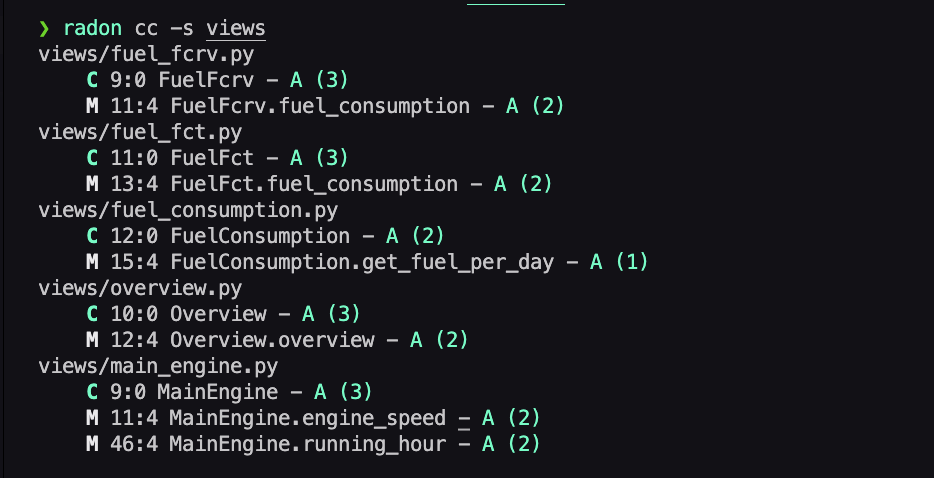
\includegraphics[width=1\linewidth, center]{images/hasil/cc-result.png}
    \caption{Hasil Perhitungan Cyclomatic Complexity}
    \label{fig:cc-result}
\end{figure}

% \begin{landscape}
%     \subsection{Blackbox Testing}

%     \subsubsection{Iterasi 1}
%     \begin{longtable}[!h]
    {
            p{0.2\textwidth}
            p{0.3\textwidth}
            p{0.3\textwidth}
            p{0.3\textwidth}
            p{0.3\textwidth}
            p{0.15\textwidth}
    }
    \caption{\textit{Blackbox Testing} Halaman Engine Speed}
    \label{tab:it1-blackbox-es} \\

    \hline
        \bfseries \textit{Test Code} &
        \bfseries \textit{Test Case} &
        \bfseries \textit{Test Steps} &
        \bfseries \textit{Expected Result} &
        \bfseries \textit{Actual Result} &
        \bfseries \textit{Pass/Fail} \\ [0.5ex]
    \hline

    \endfirsthead

    \hline
        \bfseries \textit{Test Code} &
        \bfseries \textit{Test Case} &
        \bfseries \textit{Test Steps} &
        \bfseries \textit{Expected Result} &
        \bfseries \textit{Actual Result} &
        \bfseries \textit{Pass/Fail} \\ [0.5ex]
    \hline
    \endhead % all the lines above this will be repeated on every page
    \hline

    \csvreader[
        late after line=\\,
        before reading={\catcode`\#=12},after reading={\catcode`\#=6}
    ]{tables/hasil/iterations/1/blackbox/engine-speed.csv}
    {1=\code, 2=\case, 3=\step, 4=\expect, 5=\actual, 6=\status}
    {\code & \case & \step & \expect & \actual & \status} \\

    \bottomrule
\end{longtable}
%     \newpage
%     \subsubsection{Iterasi 2}
%     \begin{longtable}[!h]
    {
            p{0.2\textwidth}
            p{0.3\textwidth}
            p{0.3\textwidth}
            p{0.3\textwidth}
            p{0.3\textwidth}
            p{0.15\textwidth}
    }
    \caption{Blackbox Testing Halaman Fuel Consumption}
    \label{tab:it1-blackbox-fc} \\

    \hline
        \bfseries \textit{Test Code} &
        \bfseries \textit{Test Case} &
        \bfseries \textit{Test Steps} &
        \bfseries \textit{Expected Result} &
        \bfseries \textit{Actual Result} &
        \bfseries \textit{Pass/Fail} \\ [0.5ex]
    \hline

    \endfirsthead

    \hline
        \bfseries \textit{Test Code} &
        \bfseries \textit{Test Case} &
        \bfseries \textit{Test Steps} &
        \bfseries \textit{Expected Result} &
        \bfseries \textit{Actual Result} &
        \bfseries \textit{Pass/Fail} \\ [0.5ex]
    \hline
    \endhead % all the lines above this will be repeated on every page
    \hline

    \csvreader[
        late after line=\\,
        before reading={\catcode`\#=12},after reading={\catcode`\#=6}
    ]{tables/hasil/iterations/2/blackbox/fuel-cons.csv}
    {1=\code, 2=\case, 3=\step, 4=\expect, 5=\actual, 6=\status}
    {\code & \case & \step & \expect & \actual & \status} \\

    \bottomrule
\end{longtable}
%     \newpage
%     \begin{longtable}[!h]
    {
            p{0.2\textwidth}
            p{0.3\textwidth}
            p{0.3\textwidth}
            p{0.3\textwidth}
            p{0.3\textwidth}
            p{0.15\textwidth}
    }
    \caption{Blackbox Testing Halaman Running Hour}
    \label{tab:it1-blackbox-rh} \\

    \hline
        \bfseries \textit{Test Code} &
        \bfseries \textit{Test Case} &
        \bfseries \textit{Test Steps} &
        \bfseries \textit{Expected Result} &
        \bfseries \textit{Actual Result} &
        \bfseries \textit{Pass/Fail} \\ [0.5ex]
    \hline

    \endfirsthead

    \hline
        \bfseries \textit{Test Code} &
        \bfseries \textit{Test Case} &
        \bfseries \textit{Test Steps} &
        \bfseries \textit{Expected Result} &
        \bfseries \textit{Actual Result} &
        \bfseries \textit{Pass/Fail} \\ [0.5ex]
    \hline
    \endhead % all the lines above this will be repeated on every page
    \hline

    \csvreader[
        late after line=\\,
        before reading={\catcode`\#=12},after reading={\catcode`\#=6}
    ]{tables/hasil/iterations/2/blackbox/running-hour.csv}
    {1=\code, 2=\case, 3=\step, 4=\expect, 5=\actual, 6=\status}
    {\code & \case & \step & \expect & \actual & \status} \\

    \bottomrule
\end{longtable}
%     \begin{longtable}[!h]
    {
            p{0.2\textwidth}
            p{0.3\textwidth}
            p{0.3\textwidth}
            p{0.3\textwidth}
            p{0.3\textwidth}
            p{0.15\textwidth}
    }
    \caption{Blackbox Testing Halaman Data Log}
    \label{tab:it1-blackbox-dl} \\

    \hline
        \bfseries \textit{Test Code} &
        \bfseries \textit{Test Case} &
        \bfseries \textit{Test Steps} &
        \bfseries \textit{Expected Result} &
        \bfseries \textit{Actual Result} &
        \bfseries \textit{Pass/Fail} \\ [0.5ex]
    \hline

    \endfirsthead

    \hline
        \bfseries \textit{Test Code} &
        \bfseries \textit{Test Case} &
        \bfseries \textit{Test Steps} &
        \bfseries \textit{Expected Result} &
        \bfseries \textit{Actual Result} &
        \bfseries \textit{Pass/Fail} \\ [0.5ex]
    \hline
    \endhead % all the lines above this will be repeated on every page
    \hline

    \csvreader[
        late after line=\\,
        before reading={\catcode`\#=12},after reading={\catcode`\#=6}
    ]{tables/hasil/iterations/2/blackbox/data-log.csv}
    {1=\code, 2=\case, 3=\step, 4=\expect, 5=\actual, 6=\status}
    {\code & \case & \step & \expect & \actual & \status} \\

    \bottomrule
\end{longtable}
%     \subsubsection{Iterasi 3}
%     \begin{longtable}[!h]
  {
          p{0.2\textwidth}
          p{0.3\textwidth}
          p{0.3\textwidth}
          p{0.3\textwidth}
          p{0.3\textwidth}
          p{0.15\textwidth}
  }
  \caption{\textit{Blackbox Testing} Halaman FCRV}
  \label{tab:it3-blackbox-fcrv} \\

  \hline
      \bfseries \textit{Test Code} &
      \bfseries \textit{Test Case} &
      \bfseries \textit{Test Steps} &
      \bfseries \textit{Expected Result} &
      \bfseries \textit{Actual Result} &
      \bfseries \textit{Pass/Fail} \\ [0.5ex]
  \hline

  \endfirsthead

  \hline
      \bfseries \textit{Test Code} &
      \bfseries \textit{Test Case} &
      \bfseries \textit{Test Steps} &
      \bfseries \textit{Expected Result} &
      \bfseries \textit{Actual Result} &
      \bfseries \textit{Pass/Fail} \\ [0.5ex]
  \hline
  \endhead % all the lines above this will be repeated on every page
  \hline

  \csvreader[
      late after line=\\,
      before reading={\catcode`\#=12},after reading={\catcode`\#=6}
  ]{tables/hasil/iterations/3/blackbox/user.csv}
  {1=\code, 2=\case, 3=\step, 4=\expect, 5=\actual, 6=\status}
  {\code & \case & \step & \expect & \actual & \status} \\

  \bottomrule
\end{longtable}
%     \begin{longtable}[!h]
    {
            p{0.2\textwidth}
            p{0.3\textwidth}
            p{0.3\textwidth}
            p{0.3\textwidth}
            p{0.3\textwidth}
            p{0.15\textwidth}
    }
    \caption{Blackbox Testing Halaman User Management}
    \label{tab:it2-blackbox-user} \\

    \hline
        \bfseries \textit{Test Code} &
        \bfseries \textit{Test Case} &
        \bfseries \textit{Test Steps} &
        \bfseries \textit{Expected Result} &
        \bfseries \textit{Actual Result} &
        \bfseries \textit{Pass/Fail} \\ [0.5ex]
    \hline

    \endfirsthead

    \hline
        \bfseries \textit{Test Code} &
        \bfseries \textit{Test Case} &
        \bfseries \textit{Test Steps} &
        \bfseries \textit{Expected Result} &
        \bfseries \textit{Actual Result} &
        \bfseries \textit{Pass/Fail} \\ [0.5ex]
    \hline
    \endhead % all the lines above this will be repeated on every page
    \hline

    \csvreader[
        late after line=\\,
        before reading={\catcode`\#=12},after reading={\catcode`\#=6}
    ]{tables/hasil/iterations/3/blackbox/user.csv}
    {1=\code, 2=\case, 3=\step, 4=\expect, 5=\actual, 6=\status}
    {\code & \case & \step & \expect & \actual & \status} \\

    \bottomrule
\end{longtable}
%     \newpage
%     \begin{longtable}[!h]
    {
            p{0.2\textwidth}
            p{0.3\textwidth}
            p{0.3\textwidth}
            p{0.3\textwidth}
            p{0.3\textwidth}
            p{0.15\textwidth}
    }
    \caption{Blackbox Testing Halaman Vessel Management}
    \label{tab:it3-blackbox-vessel} \\

    \hline
        \bfseries \textit{Test Code} &
        \bfseries \textit{Test Case} &
        \bfseries \textit{Test Steps} &
        \bfseries \textit{Expected Result} &
        \bfseries \textit{Actual Result} &
        \bfseries \textit{Pass/Fail} \\ [0.5ex]
    \hline

    \endfirsthead

    \hline
        \bfseries \textit{Test Code} &
        \bfseries \textit{Test Case} &
        \bfseries \textit{Test Steps} &
        \bfseries \textit{Expected Result} &
        \bfseries \textit{Actual Result} &
        \bfseries \textit{Pass/Fail} \\ [0.5ex]
    \hline
    \endhead % all the lines above this will be repeated on every page
    \hline

    \csvreader[
        late after line=\\,
        before reading={\catcode`\#=12},after reading={\catcode`\#=6}
    ]{tables/hasil/iterations/3/blackbox/vessel.csv}
    {1=\code, 2=\case, 3=\step, 4=\expect, 5=\actual, 6=\status}
    {\code & \case & \step & \expect & \actual & \status} \\

    \bottomrule
\end{longtable}
%     \begin{longtable}[!h]
  {
          p{0.2\textwidth}
          p{0.3\textwidth}
          p{0.3\textwidth}
          p{0.3\textwidth}
          p{0.3\textwidth}
          p{0.15\textwidth}
  }
  \caption{\textit{Blackbox Testing} Halaman FCRV}
  \label{tab:it3-blackbox-fcrv} \\

  \hline
      \bfseries \textit{Test Code} &
      \bfseries \textit{Test Case} &
      \bfseries \textit{Test Steps} &
      \bfseries \textit{Expected Result} &
      \bfseries \textit{Actual Result} &
      \bfseries \textit{Pass/Fail} \\ [0.5ex]
  \hline

  \endfirsthead

  \hline
      \bfseries \textit{Test Code} &
      \bfseries \textit{Test Case} &
      \bfseries \textit{Test Steps} &
      \bfseries \textit{Expected Result} &
      \bfseries \textit{Actual Result} &
      \bfseries \textit{Pass/Fail} \\ [0.5ex]
  \hline
  \endhead % all the lines above this will be repeated on every page
  \hline

  \csvreader[
      late after line=\\,
      before reading={\catcode`\#=12},after reading={\catcode`\#=6}
  ]{tables/hasil/iterations/3/blackbox/user.csv}
  {1=\code, 2=\case, 3=\step, 4=\expect, 5=\actual, 6=\status}
  {\code & \case & \step & \expect & \actual & \status} \\

  \bottomrule
\end{longtable}
%     \begin{longtable}[!h]
  {
          p{0.2\textwidth}
          p{0.3\textwidth}
          p{0.3\textwidth}
          p{0.3\textwidth}
          p{0.3\textwidth}
          p{0.15\textwidth}
  }
  \caption{\textit{Blackbox Testing} Halaman FCRV}
  \label{tab:it3-blackbox-fcrv} \\

  \hline
      \bfseries \textit{Test Code} &
      \bfseries \textit{Test Case} &
      \bfseries \textit{Test Steps} &
      \bfseries \textit{Expected Result} &
      \bfseries \textit{Actual Result} &
      \bfseries \textit{Pass/Fail} \\ [0.5ex]
  \hline

  \endfirsthead

  \hline
      \bfseries \textit{Test Code} &
      \bfseries \textit{Test Case} &
      \bfseries \textit{Test Steps} &
      \bfseries \textit{Expected Result} &
      \bfseries \textit{Actual Result} &
      \bfseries \textit{Pass/Fail} \\ [0.5ex]
  \hline
  \endhead % all the lines above this will be repeated on every page
  \hline

  \csvreader[
      late after line=\\,
      before reading={\catcode`\#=12},after reading={\catcode`\#=6}
  ]{tables/hasil/iterations/3/blackbox/user.csv}
  {1=\code, 2=\case, 3=\step, 4=\expect, 5=\actual, 6=\status}
  {\code & \case & \step & \expect & \actual & \status} \\

  \bottomrule
\end{longtable}
%     \newpage
%     \subsubsection{Iterasi 4}
%     \begin{longtable}[!h]
    {
            p{0.2\textwidth}
            p{0.3\textwidth}
            p{0.3\textwidth}
            p{0.3\textwidth}
            p{0.3\textwidth}
            p{0.15\textwidth}
    }
    \caption{\textit{Blackbox Testing Generate Engine Speed Daily Report}}
    \label{tab:it4-blackbox-generate-es-report} \\

    \hline
        \bfseries \textit{Test Code} &
        \bfseries \textit{Test Case} &
        \bfseries \textit{Test Steps} &
        \bfseries \textit{Expected Result} &
        \bfseries \textit{Actual Result} &
        \bfseries \textit{Pass/Fail} \\ [0.5ex]
    \hline

    \endfirsthead

    \hline
        \bfseries \textit{Test Code} &
        \bfseries \textit{Test Case} &
        \bfseries \textit{Test Steps} &
        \bfseries \textit{Expected Result} &
        \bfseries \textit{Actual Result} &
        \bfseries \textit{Pass/Fail} \\ [0.5ex]
    \hline
    \endhead % all the lines above this will be repeated on every page
    \hline

    \csvreader[
        late after line=\\,
        before reading={\catcode`\#=12},after reading={\catcode`\#=6}
    ]{tables/hasil/iterations/4/blackbox/generate-es-report.csv}
    {1=\code, 2=\case, 3=\step, 4=\expect, 5=\actual, 6=\status}
    {\code & \case & \step & \expect & \actual & \status} \\

    \bottomrule
\end{longtable}
%     \newpage
%     \begin{longtable}[!h]
    {
            p{0.2\textwidth}
            p{0.3\textwidth}
            p{0.3\textwidth}
            p{0.3\textwidth}
            p{0.3\textwidth}
            p{0.15\textwidth}
    }
    \caption{\textit{Blackbox Testing Generate Fuel Consumption Daily Report}}
    \label{tab:it4-blackbox-generate-fuel-report} \\

    \hline
        \bfseries \textit{Test Code} &
        \bfseries \textit{Test Case} &
        \bfseries \textit{Test Steps} &
        \bfseries \textit{Expected Result} &
        \bfseries \textit{Actual Result} &
        \bfseries \textit{Pass/Fail} \\ [0.5ex]
    \hline

    \endfirsthead

    \hline
        \bfseries \textit{Test Code} &
        \bfseries \textit{Test Case} &
        \bfseries \textit{Test Steps} &
        \bfseries \textit{Expected Result} &
        \bfseries \textit{Actual Result} &
        \bfseries \textit{Pass/Fail} \\ [0.5ex]
    \hline
    \endhead % all the lines above this will be repeated on every page
    \hline

    \csvreader[
        late after line=\\,
        before reading={\catcode`\#=12},after reading={\catcode`\#=6}
    ]{tables/hasil/iterations/4/blackbox/generate-fuel-report.csv}
    {1=\code, 2=\case, 3=\step, 4=\expect, 5=\actual, 6=\status}
    {\code & \case & \step & \expect & \actual & \status} \\

    \bottomrule
\end{longtable}
%     \newpage
%     \subsubsection{Iterasi 5}
%     \begin{longtable}[!h]
    {
            p{0.2\textwidth}
            p{0.3\textwidth}
            p{0.3\textwidth}
            p{0.3\textwidth}
            p{0.3\textwidth}
            p{0.15\textwidth}
    }
    \caption{Blackbox Testing Ekspor Data Log Kecepatan Mesin}
    \label{tab:it4-blackbox-generate-es-report} \\

    \hline
        \bfseries \textit{Test Code} &
        \bfseries \textit{Test Case} &
        \bfseries \textit{Test Steps} &
        \bfseries \textit{Expected Result} &
        \bfseries \textit{Actual Result} &
        \bfseries \textit{Pass/Fail} \\ [0.5ex]
    \hline

    \endfirsthead

    \hline
        \bfseries \textit{Test Code} &
        \bfseries \textit{Test Case} &
        \bfseries \textit{Test Steps} &
        \bfseries \textit{Expected Result} &
        \bfseries \textit{Actual Result} &
        \bfseries \textit{Pass/Fail} \\ [0.5ex]
    \hline
    \endhead % all the lines above this will be repeated on every page
    \hline

    \csvreader[
        late after line=\\,
        before reading={\catcode`\#=12},after reading={\catcode`\#=6}
    ]{tables/hasil/iterations/5/blackbox/export-data.csv}
    {1=\code, 2=\case, 3=\step, 4=\expect, 5=\actual, 6=\status}
    {\code & \case & \step & \expect & \actual & \status} \\

    \bottomrule
\end{longtable}

% \end{landscape}

% \section{\textit{Source Code}}

% \begin{enumerate}
%     \item \href{https://github.com}{Frontend Halaman Engine Speed}
%     \item \href{https://github.com}{Frontend Halaman Overview}
%     \item \href{https://github.com}{Frontend Halaman Fuel Consumption}
%     \item \href{https://github.com}{Frontend Halaman OP41 Report}
%     \item \href{https://github.com}{Frontend Halaman Running Hour}
%     \item \href{https://github.com}{Frontend Halaman Data Log}
%     \item \href{https://github.com}{Backend Overview}
%     \item \href{https://github.com}{Backend Engine Speed}
%     \item \href{https://github.com}{Backend Halaman Fuel Consumption}
%     \item \href{https://github.com}{Backend Halaman OP41 Report}
%     \item \href{https://github.com}{Backend Halaman Running Hour}
%     \item \href{https://github.com}{Backend Halaman Data Log}
% \end{enumerate}